\documentclass{amsart}
\usepackage{amsmath,amsthm}
\usepackage{amsfonts,amssymb}
\usepackage{accents}
\usepackage{enumerate}
\usepackage{accents,color}
\usepackage{graphicx}
\usepackage{todonotes}
\usepackage{bm}

\hfuzz1pc
%\usepackage[notref,notcite]{showkeys}

\addtolength{\textwidth}{0.5cm}

\newcommand{\lvt}{\left|\kern-1.35pt\left|\kern-1.3pt\left|}
\newcommand{\rvt}{\right|\kern-1.3pt\right|\kern-1.35pt\right|}
%%%%%%%%%%%%%%Theorem environments%%%%%%%%%%%%%%%%%%%%

%% \theoremstyle{plain} %% This is the default
\newtheorem{thm}{Theorem}[section]
\newtheorem{cor}[thm]{Corollary}
\newtheorem{lem}[thm]{Lemma}
\newtheorem{prop}[thm]{Proposition}
\newtheorem{exam}[thm]{Example}
\newtheorem{ax}{Axiom}
\newtheorem{defn}[thm]{Definition}
       

\theoremstyle{remark}
\newtheorem{rem}{Remark}[section]\newtheorem*{notation}{Notation}

\renewcommand{\theequation}{\thesection.\arabic{equation}}

\newcommand{\thmref}[1]{Theorem~\ref{#1}}
\newcommand{\secref}[1]{\S\ref{#1}}
\newcommand{\lemref}[1]{Lemma~\ref{#1}}

%%%%%%%%%%%%%%%%% Math definitions %%%%%%%%%%%%%%%%%%
 \def\la{{\langle}}
 \def\ra{{\rangle}}
 \def\ve{{\varepsilon}}

 \def\d{\mathrm{d}}
 
 \def\sph{{\mathbb{S}^{d-1}}}
 
 \def\sB{{\mathsf B}}
 \def\sC{{\mathsf C}}
 \def\sD{{\mathsf D}}
 \def\sG{{\mathsf G}}
 \def\sH{{\mathsf H}}
 \def\sK{{\mathsf K}}
 \def\sM{{\mathsf M}}
 \def\sP{{\mathsf P}}
 \def\sQ{{\mathsf Q}}
 \def\sU{{\mathsf U}}
 
 \def\ff{{\mathfrak f}}
 \def\fh{{\mathfrak h}}
 \def\fp{{\mathfrak p}}
 \def\fs{{\mathfrak s}}
 \def\fS{{\mathfrak S}}
  
 \def\a{{\alpha}}
 \def\b{{\beta}}
 \def\g{{\gamma}}
 \def\k{{\kappa}}
 \def\t{{\theta}}
 \def\l{{\lambda}}
 \def\o{{\omega}}
 \def\s{\sigma}
 \def\la{{\langle}}
 \def\ra{{\rangle}}
 \def\ve{{\varepsilon}}
 \def\ab{{\mathbf a}}
 \def\bb{{\mathbf b}}
 \def\cb{{\mathbf c}}
 \def\ib{{\mathbf i}}
 \def\jb{{\mathbf j}}
 \def\kb{{\mathbf k}}
 \def\lb{{\mathbf l}}
 \def\mb{{\mathbf m}}
  \def\nb{{\mathbf n}}
 \def\rb{{\mathbf r}}
 \def\sb{{\mathbf s}}
 \def\tb{{\mathbf t}}
 \def\ub{{\mathbf u}}
 \def\vb{{\mathbf v}}
 \def\xb{{\mathbf x}}
 \def\yb{{\mathbf y}}
 \def\Ab{{\mathbf A}}
  \def\Bb{{\mathbf B}}
 \def\Db{{\mathbf D}}
 \def\Eb{{\mathbf E}}
 \def\Fb{{\mathbf F}}
 \def\Gb{{\mathbf G}}
 \def\Kb{{\mathbf K}}
 \def\Pb{{\mathbf P}}
 \def\CB{{\mathcal B}}
 \def\CD{{\mathcal D}}
 \def\CF{{\mathcal F}}
 \def\CH{{\mathcal H}}
 \def\CI{{\mathcal I}}
 \def\CJ{{\mathcal J}}
 \def\CL{{\mathcal L}}
 \def\CO{{\mathcal O}}
 \def\CP{{\mathcal P}}
 \def\CM{{\mathcal M}}
 \def\CT{{\mathcal T}}
 \def\CU{{\mathcal U}}
 \def\CV{{\mathcal V}}
 \def\CA{{\mathcal A}}
 \def\CW{{\mathcal W}}
 \def\BB{{\mathbb B}}
 \def\CC{{\mathbb C}}
 \def\KK{{\mathbb K}}
 \def\NN{{\mathbb N}}
 \def\PP{{\mathbb P}}
 \def\QQ{{\mathbb Q}}
 \def\RR{{\mathbb R}}
 \def\SS{{\mathbb S}}
 \def\VV{{\mathbb V}}
 \def\TT{{\mathbb T}}
 \def\YY{{\mathbb Y}}
 \def\ZZ{{\mathbb Z}}
      \def\proj{\operatorname{proj}}
      \def\Lip{\operatorname{Lip}}
      \def\vi{\varphi}
\def\lla{\langle{\kern-2.5pt}\langle}      
\def\rra{\rangle{\kern-2.5pt}\rangle}      

\newcommand{\wt}{\widetilde}
\newcommand{\wh}{\widehat}
\def\rhow{{\lceil\tfrac{\varrho}{2}\rceil}}
\newcommand{\rhoh}{{\lfloor\tfrac{\varrho}{2}\rfloor}}

\DeclareMathOperator{\IM}{Im}
\DeclareMathOperator{\esssup}{ess\,sup}
\DeclareMathOperator{\meas}{meas}

\def\brho{{\boldsymbol{\rho}}}

\def\f{\frac}
\def\va{\varepsilon}
\def\sub{\substack}

\newcommand{\sotodo}{\todo[color=green]}
\newcommand{\sotodoinline}{\todo[color=green,inline=true]}


\graphicspath{{./}}
\begin{document}

\title{Orthogonal polynomials on planar cubic curves}

\author{Marco Fasondini}
\address{Department of Mathematics\\
Imperial College\\
 London \\
 United Kingdom  }\email{m.fasondini@imperial.ac.uk}

\author{Sheehan Olver}
\address{Department of Mathematics\\
Imperial College\\
 London \\
 United Kingdom  }\email{s.olver@imperial.ac.uk}

\author{Yuan Xu}
\address{Department of Mathematics\\ University of Oregon\\
    Eugene, Oregon 97403-1222.}\email{yuan@uoregon.edu}

\date{\today}
\keywords{orthogonal polynomials, orthogonal series }
\subjclass[2010]{ 33C50, 35C10, 42C05, 42C10}

\begin{abstract} 
  
\end{abstract}
\maketitle
 
\section{Introduction}
\setcounter{equation}{0}
 
We study orthogonal polynomials of two variables with respect to an inner product defined on a cubic curve. The
admissible cubic curves are of the form $y^2 = \phi(x)$, where $\phi$ is a cubic polynomial of one variable. This
family of curves includes the standard elliptic curves. 
.....
 
\section{Orthogonal polynomials on cubic curves}
\setcounter{equation}{0}

\subsection{Cubic curves}\label{sect:cubiccurves}
Throughout this paper we let $\phi$ be a cubic polynomial defined by 
\begin{equation}\label{eq:cubic-curve}
  \phi(x) = a_0 x^3 + a_1 x^2 + a_2 x + a_3, \qquad a_i \in \RR, \quad a_0 \ne 0.
\end{equation}
We consider the cubic curve $\g$ on the plane defined by 
$$
    y^2 = \phi(x), \qquad (x,y) \in \RR^2,  
$$
and $\g = \{(x,y): y^2 = \phi(x)\}$ is the graph of the curve. Without loss of generality, we assume that 
$a_0>0$, so that $\phi(x) > 0$ for sufficiently large $x > 0$. Let 
$$
   \Omega_\g:= \{x: \phi(x) \ge 0\},
$$
which is the set on which the cubic curve is defined. The cubic polynomial $\phi$ can have either one 
real zero of three real zeros, so that $\Omega_\g$ can be either one interval or the union of two
intervals. This leads to three possibilities: 
\begin{enumerate}[    (I)]
\item $\Omega_\g = [A,\infty)$: the curve has one component; 
\item $\Omega_\g = [A_1, B_1] \cup [A_2, \infty)$: the curve has two components; 
\item $\Omega_\g = [A,B]$: the curve has one component and is a closed curve.
\end{enumerate}
In the first case, $\phi$ has one real zero $A$. In the second case, $\phi$ has three real
zeros $A_1 < B_1 < A_2$. In the third case, $\phi$ has three real zeros $A < B = B$ or a
double zero at $B$. 
For examples, see Figures 1 and 2 below. 

One important family of cubic curves included in our definition is that of {\it elliptic curves}. 
Recall that an elliptic curve is a plane curve defined by 
\begin{equation} \label{eq:elliptic1}
     y^2 = x^3 + a x + b, 
\end{equation}
where $a$ and $b$ are real numbers and the curve has no-cusps, self-intersections, or isolated points. This 
holds if and only if the discriminant
$$
\Delta_E = -16(4a^{3}+27b^{2})
$$
is not equal to zero. The graph has two components if $\Delta_E > 0$ and one component if $\Delta_E < 0$.
Two elliptic curves are depicted in Figure 1, the lefthand one has one component, whereas the righthand one 
has two components. 
\begin{figure}[ht]
  \begin{center}
    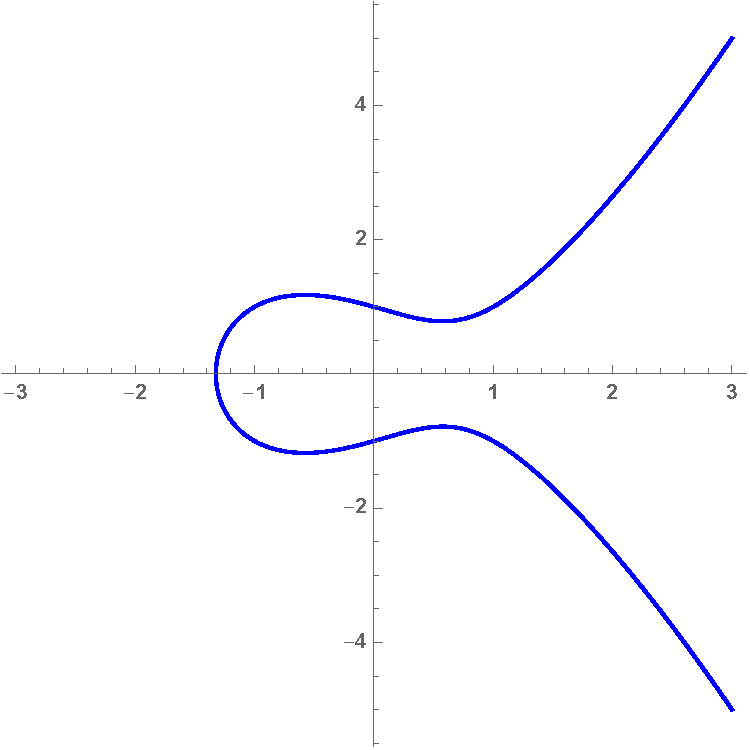
\includegraphics[width=0.45\textwidth]{elliptic1} \qquad 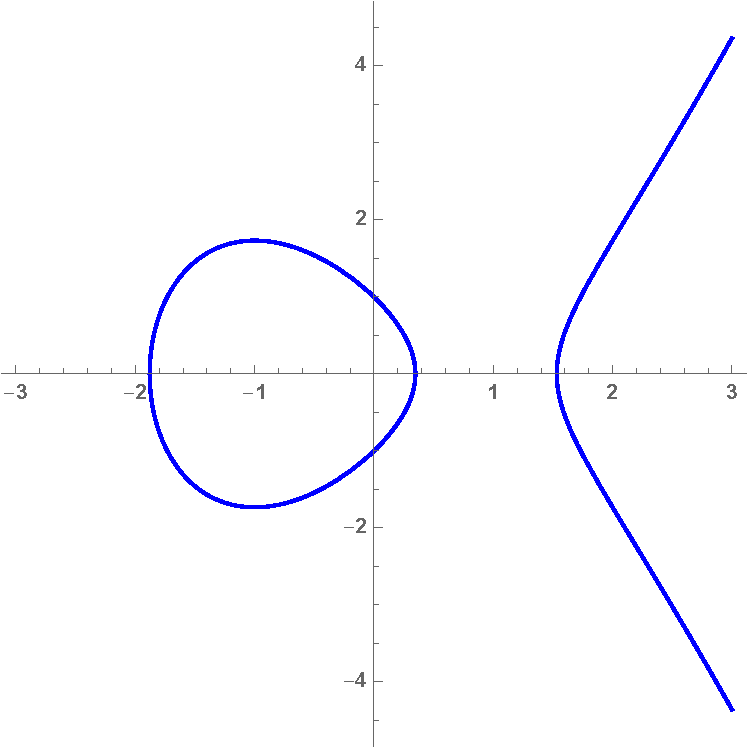
\includegraphics[width=0.45\textwidth]{elliptic2}
  \end{center} 
  \caption{Elliptic curves. Left: $y^2=x^3-x+1$. Right: $y^2=x^3-3x+1$}
\end{figure}

We can write the elliptic curve in a different form. Let $\phi(x) = x^3 + a x + b$. By the definition, $\phi(A) = 0$ 
or $b = - A^3 - a A$, so that 
$$
  \phi(x) =  x^3 + a x - A^3 - a A = (x-A) (x^2 + A x +A^2+a). 
$$
We need $x^2 + A x + A^2 + a \ge 0$ for $x \ge A$, which holds only if its discriminant $A^2- 4 (A^2+a) < 0$ 
or $a > - (3/4)A^2$. Under this condition, we have 
$$
 4 a^3 + 27 b^2 = 4 a^3 + 27 A^2 (A^2+a)^2 > - 4 \frac{3^3}{4^3} A^6 +27 A^2 \left(\frac{A^2}{4}\right)^2 = 0,
$$ 
so that the elliptic curve does indeed have one component. Thus, setting $c = a + \frac{3}{4}A^2$ and 
$b = - A^3 - a A$ we see that the elliptic curve \eqref{eq:elliptic1} becomes 
\begin{equation} \label{eq:elliptic2}
      y^2 = (x-A) \left( \left (x+\tfrac{A}{2}\right)^2 + c\right), \qquad A\in \RR.
\end{equation}
If $c > 0$, then $\phi(x) = (x-A) (x+\frac{A}{2})^2 + c$ has one real zero, so that the elliptic curve has one
component. If $c < 0$, then the curve has two components. One of advantages of this writing the curve in 
the form of \eqref{eq:elliptic2} is that the roots of $\phi$ are explicitly given. 

We also consider cubic curves that are not elliptic. For example, we can have cubic curves of the form $y^2 = a (x^3 - b x^2)$, which will be self intersect 
when $b>0$, which we can treat as two components that touch at one pint. One example of such curves is depicted in Figure 2. 

As an example of the third case, that of closed cubic curves, we mention tear drop curves defined by 
$$
     (2a)^2 y^2 = (x-a)^2 (x+a), \qquad -a < x < a. 
$$
For $a=1$, this curve is inside the unit circle and is depicted in Figure 2. 
\begin{figure}[ht]
  \begin{center}
    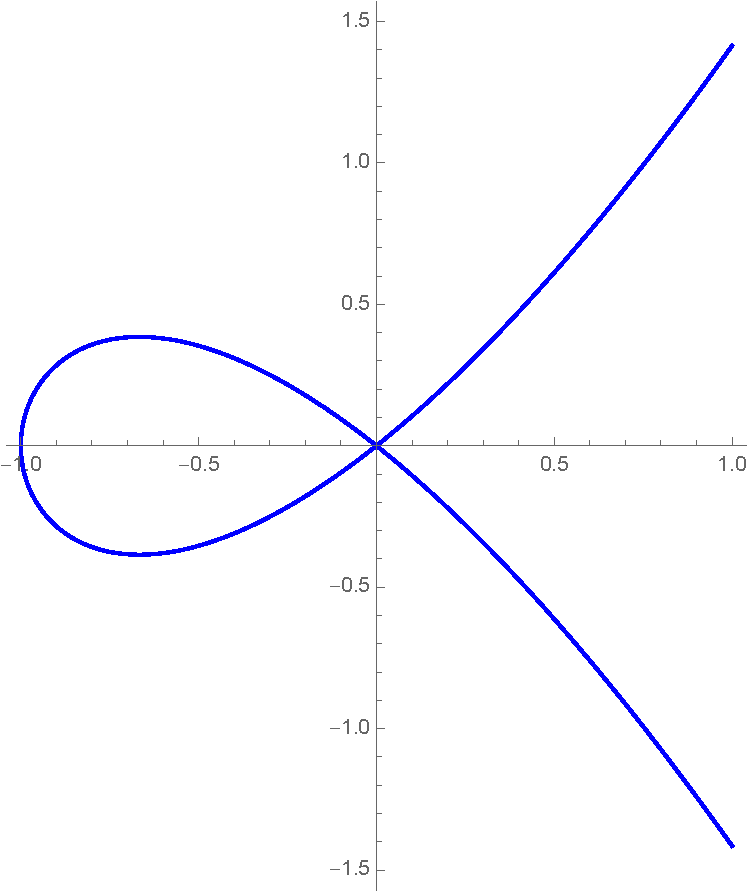
\includegraphics[width=0.38\textwidth]{elliptic3} \qquad\quad  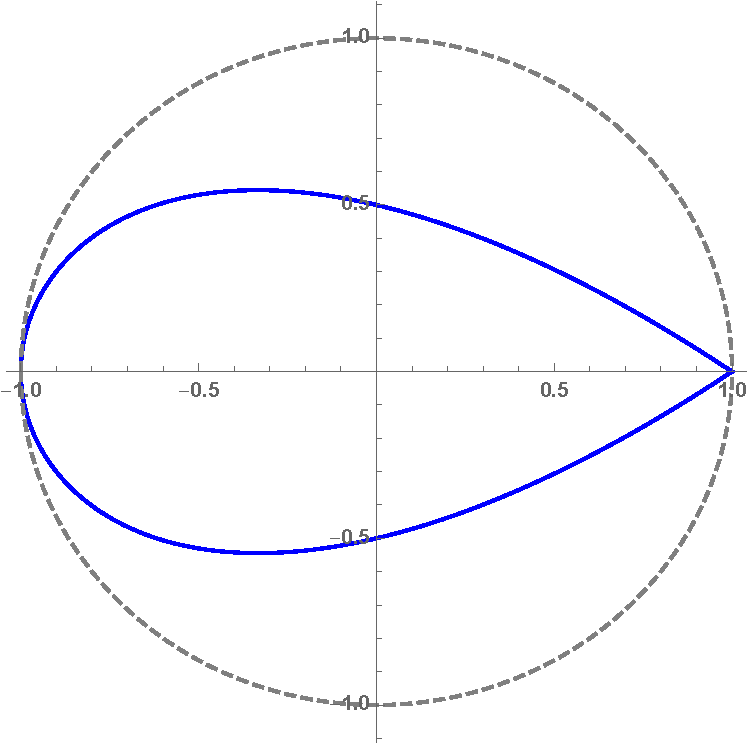
\includegraphics[width=0.45\textwidth]{teardrop}
  \end{center} 
  \caption{Left:  $y^2= x^2(x+1)$. Right:  the tear drop curve $4 y^2= (1-x)^2 (1+x)$}
\end{figure}

Our definition also include the curve $y^2 = x^3$, which is the case of $a= b = 0$ in \eqref{eq:elliptic1},
but the curve has a singular point and is not an elliptic curve. 

\subsection{Orthogonal polynomials on cubic curves}
Let $y^2=\phi(x)$ be a cubic curve and let $w$ be a non-negative weight function defined on $\Omega_\g$. 
We consider orthogonal polynomials of two variables that are orthogonal with respect to an inner product 
defined, on an appropriate polynomial subspace, by 
\begin{equation} \label{eq:ipd1}
  \la f,g\ra_{\g,w} = \int_{\g} f(x,y) g(x,y) w(x) \d \s(x,y),
\end{equation}
where $\d \s$ is the arc length measure on the curve. Depending on the support set of $w$, the integral
domain could be compact in the cases I and II. 

The bilinear form $\la \cdot,\cdot\ra_{\g,w}$ defines an inner product on the space $\RR[x,y] / \la y^2 - \phi(x)\ra$. 
For $n\ge 3$, the monomials of degree exactly $n$, $x^k y^{n-k}$ for $0 \le k \le n$, remain of degree $n$ 
after mod the ring $\la y^2 - \phi(x)\ra$ only when $k =0,1,2$. In particular, this shows that 
$\CB_n = \{y^n, x y ^{n-1}, x^2 y^{n-2}\}$ is a basis of the space of polynomials of degree exactly $n$ in 
$\RR[x,y] / \la y^2 - \phi(x)\ra$. 

Let $\CV_n:=\CV_n(\g,w)$ be the space of orthogonal polynomials of degree $n$ in two variables with respect to this 
inner product. Applying the Gram-Schmidt process to the basis $\CB_n$, for example, inductively on $n$, 
we obtain the following proposition:

\begin{prop}\label{prop:dimVn}
For $n \in \NN_0$, we have $\dim \CV_0 =1$, $\dim \CV_1 =2$ and 
$$
   \dim \CV_n =3, \quad n \ge 2.
$$
\end{prop}

A basis of $\CV_n$ can be given explicitly in terms of orthogonal polynomials with respect to $w$ and $\phi w$.
We can write the inner product $\la \cdot,\cdot\ra_{\g,w}$ as 
\begin{align} \label{eq:ipd2}
  \la f,g \ra_{\g,w} = \int_{\Omega_\g} & \left[  f\left(x, \sqrt{\phi(x)} \right) g\left(x, \sqrt{\phi(x)} \right) \right. \\
      & \left. + f\left(x, - \sqrt{\phi(x)} \right) g\left(x, -\sqrt{\phi(x)} \right)\right] w(x) \d x. \notag
\end{align}
More precisely, the domain $\Omega_\g$ in the integral should be replaced by $\Omega_\g \cap \mathrm{supp}(w)$,
where $\mathrm{supp}(w)$ denotes the support set of $w$. For example, in case $I$, we could choose $w$ 
so that it has support set $[A,B]$ for some $B \in \RR$. 

Let $p_n(w)$ be usual orthogonal polynomial with respect to $w$ on $\Omega_\g$ for a generic $w$. In particular,
$p_n(\phi w)$ stand for orthogonal polynomials with respect to $\phi(x) w(x)$ on $\Omega_\g$. We now define an 
explicit basis for the space $\CV_n(w)$ of orthogonal polynomials on the cubic curve $\g$. We denote this basis by 
$Y_{n,i}$ and denote its norm by $H_{n,i}$. 
 
\begin{thm} \label{thm:OPbasis}
Let $\g$ be a cubic curve and let $w$ be a weight function defined on $\Omega_\g$.
\begin{enumerate}[1.]
\item For $n =0$ and $n=1$, we define
$$
Y_0(x,y) =1, \qquad Y_{1,1}(x,y) = p_1(w;x), \qquad Y_{1,2}(x,y)=y.
$$
Then $\CV_0 = \mathrm{span} \{Y_0\}$ and $\CV_1 =  \mathrm{span} \{Y_{1,1}, Y_{1,2}\}$. Moreover,
$$
   H_0 = 2 h_0(w), \qquad H_{1,1} = 2 h_1(w), \qquad H_{1,2} = 2 h_0(\phi w).
$$
\item For $m \in \NN_0$ and $m \ge 1$, we define 
\begin{align*}
  Y_{2m,1}(x,y) &\, = p_{3m}(w;x), \\
  Y_{2m,2}(x,y) &\,= p_{3m-1}(w;x), \\
  Y_{2m,3}(x,y) &\,= y p_{3m-2}(\phi w; x),
\end{align*}
and 
\begin{align*}
  Y_{2m+1,1}(x,y) &\, = p_{3m+1}(w;x), \\
  Y_{2m+1,2}(x,y) &\,= y p_{3m}(\phi w;x), \\
  Y_{2m+1,3}(x,y) &\,= y p_{3m-1}(\phi w; x).
\end{align*}
Then $Y_{n,i}$ is a polynomial of degree $n$ in $\RR[x,y] / \la y^2 - \phi(x)\ra$ for $i=1,2,3$ and
$$
\CV_n = \mathrm{span} \{Y_{n,1}, Y_{n,2}, Y_{n,3} \}, \qquad n \ge 2.
$$
Moreover,  the norms of these polynomials are given by
\begin{align*}  
H_{2m,1} & = 2 h_{3m}(w), \quad H_{2m,2} = 2 h_{3m-1}(w), \quad H_{2m,3} = 2 h_{3m-2}(\phi w),\\
H_{2m+1,1} & = 2 h_{3m+1}(w), \quad H_{2m+1,2} = 2 h_{3m}(\phi w), \quad H_{2m+1,3} = 2 h_{3m-1}(\phi w).
\end{align*}
\end{enumerate}
\end{thm}

\begin{proof}
The orthogonality in the case of $m=0$ and $1$ follows from, by the expression of $\la \cdot,\cdot\ra_{\g,w}$
in \eqref{eq:ipd2}, 
\begin{equation} \label{eq:ipd-parity}
  \la f(x), y g(x) \ra_{\g,w} = 0, 
\end{equation}
a fact that helps us to identify an orthogonal basis for $\CV_n$ for every $n \ge 2$. 

For $m \ge 2$, we first show that $Y_{n,i}$ is of degree $n$ in $\RR[x,y] / \la y^2 - \phi(x)\ra$. Throughout 
this proof, we introduce a function $\psi(x,y)$ so that the equation of the cubic curve becomes
$$
     \psi (x,y) = x^3, \qquad \psi(x,y) = a_0^{-1}( y^2 - a_1 x^2-a_2 x - a_3).
$$
Now, for $n =2m$, we write
\begin{align*}
& p_{3m}(w;x) = \sum_{k=0}^{3m} b_k x^k  = b_0 + b_1 x + \sum_{j=1}^{m} b_{3j-1} x^{3j-1} +
  \sum_{j=1}^{m} b_{3j} x^{3j} +  \sum_{j=1}^{m-1} b_{3j+1} x^{3j+1} \\
  &\qquad = b_0 + b_1 x + \sum_{j=1}^{m} b_{3j-1} (\psi(x,y))^{j-1}x^2 +
  \sum_{j=1}^{m} b_{3j} (\psi(x,y))^j + \sum_{j=1}^{m-1} b_{3j+1} x (\psi(x,y))^j, 
\end{align*}
which is a polynomial of degree $2m$ in $x,y$ variables. The same argument also shows that $p_{3m-1}(w;x)$
is a polynomial of degree $2m$ in $\RR[x,y] / \la y^2 - \phi(x)\ra$. Furthermore, it follows that $p_{3m-2}(w;x)$
is a polynomial of degree $2m-1$ in $\RR[x,y] / \la y^2 - \phi(x)\ra$, which shows that $Y_{2m,3}$ is a 
polynomial of degree $2m$ mod $ \la y^2 - \phi(x)\ra$. The similar argument works for $Y_{2m+1,i}$. 

We now verify the orthogonality. The orthogonality among some $Y_{n,i}$'s follow readily form \eqref{eq:ipd-parity}.
For the remaining cases among $Y_{2m,j}$ and $Y_{2 l +1,k}$, it is easy to see that $\la Y_{2m,1}, Y_{2l+1,1} \ra = 0$
and $\la Y_{2m,2}, Y_{2l+1,1} \ra =0$ follow immediately from the orthogonality of $p_n(w)$. Moreover, 
$$
   \la Y_{2m,3}, Y_{2l+1,2} \ra = \int_{\Omega_\g}  \phi(x) p_{3m-2}(\phi w;x) p_{3l}(\phi w;x) w(x) d x = 0
$$ 
and, similarly,  $\la Y_{2m,3}, Y_{2l+1,3} \ra =0$. Thus, we have verified that $\la Y_{2m,j}, Y_{2l+1,k}\ra = 0$
for all $l, m$ and $1\le j,k \le 3$. For $Y_{2m,j}$ and $Y_{2l,k}$, those not covered by  \eqref{eq:ipd-parity} are
$\la Y_{2m,j}, Y_{2l,k} \ra = 0$, $j, k \in \{1,2\}$, which are equal to zero by the orthogonality of $p_n(w)$ whenever
$l \ne m$ or $j \ne k$, and $\la Y_{2m,3}, Y_{2l,3} \ra$, which is equal to zero by the orthogonality of $p_n(\phi w)$. 
This shows already that $\{Y_{2m,j}: j=1,2,3\}$ is an orthogonal basis of $\CV_2m$. It is easy to see that the same consideration also shows that $\{Y_{2l+1,k}:j=1,2,3\}$ is an orthogonal basis fo $\CV_{2l+1}$. 

To determine norm of $Y_{n,i}$, we observe that if $f(x,y)= k(x)$ or $f(x,y) = y k(x)$ then 
$$
    \la f, f \ra =  \int_{\Omega_\g} [f^2(x,y)+  f^2(x,-y)] w(x) \d x = 2 \int_{\Omega_\g} f^2(x,y) w(x)\d x. 
$$
It implies, for example, $H_{2m,1}= \la Y_{2m,1},Y_{2m,1} \ra_{\g,w} = 2 h_{3m}(w)$ and
$$
H_{2m,3}= \la Y_{2m,3},Y_{2m,3} \ra_{\g,w} = 2  \int_A^B p_{3m-2}(\phi w; x) \phi^2(x) w(x)\d x = 2 h_{3m-2}(\phi w). 
$$
Norms of other polynomials are determined similarly. The proof is complete.
\end{proof}
 
We will give several examples to illustrate the result in the following section. 

\subsection{Fourier orthogonal series}
For $w$ defined on $\RR$, the Fourier orthogonal series in terms of orthogonal polynomials $\{p_n(w)\}$ is 
defined by 
$$
   f = \sum_{n=0}^\infty \wh f_n(w) p_n(w), \qquad p_n(w) = \frac{1}{h_n(w)} \int_\RR f(t) p_n(w;t) w(t) \d t,
$$
where the identity holds in $L^2(w)$ as long as polynomials are dense in $L^2(w)$, which we assume to be
the case. Furthermore, let $s_n(w;f)$ denote the $n$-th orthogonal partial sum of this expansion; that is, 
$$
 s_n(w;f) = \sum_{k=0}^n \wh f_k(w) p_k(w), \qquad n =1,2,\ldots.
$$

Likewise, let $\g$ be a cubic curve and $w$ be a weight function defined on $\g$, we define the Fourier 
orthogonal series of $f\in L^2(\g,w)$ by 
$$
  f = \wh f_0 Y_0 +  \wh f_{1,2}Y_{1,1} +  \wh f_{1,2}Y_{1,2} +
  \sum_{n=2}^\infty \sum_{i=1}^3 \wh f_{n,i} Y_{n,i} \quad\hbox{with} \quad f_{n,i} =\frac{ \la f, Y_{n,i}\ra_{\g,w}}{H_{n,i}(w)}. 
$$
The $n$-th partial sum of this expansion is denoted by $S_n(w;f)$; that is, 
$$
S_n(w; f) = \wh f_0 Y_0 +  \wh f_{1,2}Y_{1,1} +  \wh f_{1,2}Y_{1,2} +
  \sum_{k=2}^n \sum_{i=1}^3 \wh f_{k,i} Y_{k,i}.
$$
The next theorem shows that this partial sum can be written in terms of the partial sums of orthogonal 
series with respect to $w$ and $\phi w$. Let $\|\cdot\|_w$ denote the norm of $L^2(\g,w)$.

\begin{thm}
Let $\g$ be a cubic curve and let $w$ be a weight function defined on $\Omega_\g$. For $f \in 
L^2(\g,w)$, define 
\begin{align} \label{eq:fe-fo}
\begin{split}
  f_e(x):= & \frac{f\left(x, \sqrt{\phi(x)}\right)+ f\left(x, - \sqrt{\phi(x)}\right)}{2}, \\
  f_o(x):= & \frac{f\left(x, \sqrt{\phi(x)}\right)- f\left(x, - \sqrt{\phi(x)}\right)}{2 \sqrt{\phi(x)}}
\end{split}
\end{align}
for $x \in \Omega_\g$. Then
\begin{align*}
\begin{split}
  S_{2m} (w; f, x, y) &= s_{3m} (w; f_e, x) + y s_{3m-2} (w; f_o, x), \qquad (x,y) \in \g. \\
  S_{2m+1} (w; f, x, y) & = s_{3m+1} (w; f_e, x) + y s_{3m} (w; f_o, x), \qquad (x,y) \in \g.
\end{split}
\end{align*}
Furthermore, the $L^2(\g,w)$ norm of $S_n(w;f)$ satisfies
\begin{align}\label{eq:norm-partialsum}
\begin{split}
  \left \|S_{2m}(w; f)\right \|_{\g,w}^2 & = 2 \|s_{3m} (w; f_e) \|_{w}^2 +2 \| s_{3m-2} (w; f_o)\|_{\phi w}^2, \\
  \|S_{2m+1}(w; f)\|_{\g,w}^2 & = 2 \|s_{3m+1} (w; f_e) \|_{w}^2 +2 \| s_{3m} (w; f_o)\|_{\phi w}^2. 
\end{split}
\end{align}
\end{thm}

\begin{proof}
Form our definition of $f_e$ it follows immediately that 
$$
 \la f, Y_{2m,1} \ra_{\g,w} = 2 \int_{\Omega_\g}  f_e(x) p_{3m}(w;x) w(x) \d x
$$
so that, by $H_{2m,1} = 2 h_{3m}(w)$, we obtain $\wh f_{2m,1} = \{\wh f_e\}_{3m}(w)$. The same argument
shows also $\wh f_{2m,2} = \{\wh f_e\}_{3m-1}(w)$ and $\wh f_{2m+1,1} = \{\wh f_e\}_{3m+1}(w)$. Furthermore,
we also have 
\begin{align*}
 \la f, Y_{2m,3} \ra_{\g,w} & = 2 \int_{\Omega_\g}  \Big[ f\left(x,\sqrt{\phi(x)}\right) - f\left(x,- \sqrt{\phi(x)}\right) \Big]
     p_{3m-2}(\phi w;x) \sqrt{\phi(x)} w(x) \d x \\
     &  = 2 \int_{\Omega_\g}   f_o(x)  p_{3m-2}(\phi w;x) \phi(x) w(x) \d x, 
\end{align*}
so that $\wh f_{2m,3} = \{\wh f_o\}_{3m-2}(\phi w)$. The same argument also shows $\wh f_{2m+1,2} =
 \{\wh f_o\}_{3m}(\phi w)$ and $\wh f_{2m+1,3} = \{\wh f_o\}_{3m-1}(\phi w)$. Moreover, for the case 
 $m=0$ and $m=1$, we obtain $\wh f_0 = \{\wh f_e\}_0(w)$, $\wh f_{1,1} = \{\wh f_e\}_1(w)$, 
$\wh f_{1,2} = \{\wh f_o\}_0(\phi w)$, respectively. 

Setting $F_k(x) =  \{\wh f_e\}_k(w) p_k(w;x)$ and $G_k(x) =  \{\wh f_o\}_k(\phi w) p_k(\phi w;x)$, we can 
writhe the partial sum with $n = 2m$ as 
\begin{align*}
 S_{2m}(w; f)(x,y)  = & F_0(x) + F_1(x) + y G_0(x)  + \sum_{k=1}^{m} \left[G_{3k+1}(x) +F_{3k-1}(x) + y G_{3k-2} (x) \right]\\
    & + y \sum_{k=1}^{m-1} \left[F_{3k+1}(x) + y G_{3k}(x) + y G_{3k-1} (x) \right]\\
   = & \sum_{k=0}^{3m+1} F_k (x) + y \sum_{k=0}^{3m-2} G_k(x) =
   s_{3m} (w; f_e, x) + y s_{3m-2} (w; f_o, x).
\end{align*}
A similar proof works for $S_{2m+1}(w;f)$. By \eqref{eq:ipd-parity} and the Parseval identity, we see that 
\begin{align*}
 \|S_{2m}(w;f)\|_w^2 & = \|s_{3m} (w; f_e, x) \|_{\g,w}^2 + \| y s_{3m-2} (w; f_o, x)\|_{\g,w}^2 \\
      & = 2 \|s_{3m} (w; f_e) \|_{w}^2 +2 \| s_{3m-2} (w; f_o)\|_{\phi w}^2,
\end{align*}
where the second identity follows since $|s_{3m} (w; f_e, x)|^2$ does not contain $y$, whereas
$|y s_{3m} (w; f_o, x)|^2$ contains a $y^2$, which is equal to $\phi(x)$. The proof for the norm of 
$S_{2m+1}(w;f)$ is similar. This completes the proof. 
\end{proof}

\begin{cor}
Let $\g$ be a cubic curve and let $w$ be a weight function defined on $\Omega_\g$. Let $f \in 
L^2(\g)$. Then $S_n(w; f)$ converges to $f$ in $L^2(\g,w)$. 
\end{cor}

\begin{proof}
For $f\in L^2(\g,w)$, it follows from \eqref{eq:ipd2} and $|a+b|^2 \le 2 (|a|^2+|b|^2)$ that 
$$
  \|f_e\|_w^2 \le \frac12 \int_{\Omega_f} \left[|f\big (x,\sqrt{\phi(x)} \big)|^2 + |f\big (x,- \sqrt{\phi(x)} \big)|^2\right]\d x
     = \frac12 \|f\|_{\g,w}^2
$$
and similarly $\|f_o\|_{\phi w}^2 \le  \frac12 \|f\|_{\g,w}^2$. Hence, $f_e \in L^2(w)$ and $f_o \in L^2(\phi w)$. 
It follows that $s_n(w; f_e)$ converges to $f_e$ in $L^2(w)$ and $s_n(w; f_o)$ converges to 
$f_o$ in $L^2(\phi w)$. Consequently, the convergence of $S_n(w; f)$ in $L^2(\g,w)$ follows from 
\eqref{eq:norm-partialsum}.
\end{proof}

\subsection{Jacobi operators}
Let $\{Y_{n,i}\}$ be the orthonormal basis of the space $\CV_n$ defined in Theorem \ref{thm:OPbasis}.
Let $\wh Y_{n,i} = Y_{n,i}/\sqrt{H_{n,i}}$. Then $\{wh Y_{n,i}\}$ is an orthonormal basis of $\CV_n$. 
Define 
$$
   \YY_0 =\left[\wh Y_0\right], \quad \YY_1 = \left[ \begin{matrix} \wh Y_{1,1} \\ \wh Y_{1,2}  \end{matrix} \right]
    \quad \hbox{and}\quad \YY_n = \left[ \begin{matrix} \wh Y_{n,1} \\ \wh Y_{n,2} \\ \wh Y_{n,3} \end{matrix} \right], \quad n \ge 2.
$$ 
The general theorem of orthogonal polynomials of several variables shows that
\begin{align}
 x \YY_n &\, = A_{n,1} \YY_{n+1} + B_{n,1} \YY_n + A_{n-1,1}^t \YY_{n-1},  \label{eq:xrec}\\
 y \YY_n &\, = A_{n,2} \YY_{n+1} + B_{n,2} \YY_n + A_{n-1,2}^t \YY_{n-1}, \label{eq:yrec}
\end{align}
where $A_{0,i}$ are $1\times 2$ matrices and $B_{n,0}$ is a real number; $A_{1,i}$ are $2\times 3$ matrices
and $B_{1,i}$ are $2\times 2$ matrices; $A_{n,i}$ and $B_{n,i}$ are $3\times 3$ matrices for all $n \ge 2$.
The matrices $A_{n,i}$ and $B_{n,i}$ are determined by orthogonality relations: 
$$
  A_{n,i} = \la x  \YY_n \YY_{n+1}^t \ra_w, \quad A_{n,2} = \la y  \YY_n \YY_{n+1}^t \ra_w, 
  \quad  B_{n,1} = \la x  \YY_n \YY_{n}^t \ra_w, \quad B_{n,2} = \la y  \YY_n \YY_{n}^t \ra_w.
$$
In particular, by \eqref{eq:ipd-parity}, it is easy to see that these matrices are of the form
\begin{align*}
 A_{1,1}  = \, \left[\begin{matrix} 0 & \ast & 0 \\ 0 & 0 & \ast  \end{matrix}\right],
  \quad A_{2m,1}  = & \, \left[\begin{matrix} \ast & 0 & 0 \\ 0 & 0 & 0 \\ 0 & 0 & \ast  \end{matrix}\right] 
\quad \hbox{and}\quad 
A_{2m+1,1}  =  \, \left[\begin{matrix} 0 & \ast & 0 \\ 0 & 0 & \ast \\ 0 & 0 & 0 \end{matrix}\right],\quad m \ge 1 \\
B_{1,1}  =  \, \left[\begin{matrix} \ast & 0 \\ 0 & \ast  \end{matrix}\right], \quad 
B_{2m,1} = & \, \left[\begin{matrix} \ast & \ast & 0 \\ \ast & \ast & 0 \\ 0 & 0 & \ast  \end{matrix}\right]
\quad \hbox{and}\quad 
B_{2m+1,1}  =  \, \left[\begin{matrix} \ast & 0 & 0 \\ 0 & \ast & \ast \\ 0 & \ast & \ast  \end{matrix}\right], \quad m \ge 1. 
\end{align*}
and 
\begin{align*}
 A_{1,2}  = \, \left[\begin{matrix} 0& 0 & \ast \\ \ast & \ast & 0  \end{matrix}\right],
  \quad A_{2m,2}  = & \, \left[\begin{matrix} 0 & \ast & \ast \\ 0 & 0 & \ast \\ 0 & 0 & 0  \end{matrix}\right] 
\quad \hbox{and}\quad 
A_{2m+1,2}  =  \, \left[\begin{matrix} 0 & 0 & \ast \\ \ast & \ast & 0 \\ 0 & 0 & \ast  \end{matrix}\right],\quad m \ge 1 \\
B_{1,2}  =  \, \left[\begin{matrix} 0 & \ast \\ \ast & 0  \end{matrix}\right], \quad 
B_{2m,2} = & \, \left[\begin{matrix} 0& 0 & \ast \\ 0 & 0 &\ast \\ \ast & \ast & 0  \end{matrix}\right]
\quad \hbox{and}\quad 
B_{2m+1,2}  =  \, \left[\begin{matrix} 0 & \ast & \ast \\ \ast & 0 & 0 \\ \ast & 0 & 0 \end{matrix}\right], \quad m \ge 1. 
\end{align*}
These three-term relations in two variables hold when $(x,y)$ are on the cubic curve $\g$ or modulo to the 
polynomial ideal $\la y^2-\phi(x)\ra$. It is worth mentioning that we obtain, for example, 
$$
  x Y_{2m,2} = (B_{2m,1})_{2,1} Y_{2m,1} + (B_{2m,1})_{2,2} Y_{2m,2} + (A_{2m-1,1})_{2,1} Y_{2m-1,1},
$$
where $(A)_{i,j}$ stands for $(i,j)$-element of the matrix $A$, in which the lefthand side is a polynomial
of degree $n+1$, where the righthand side is of degree $n$. This holds without contradiction because 
of $(x,y) \in \g$.  

\section{Quadrature rule and polynomial interpolation}
\setcounter{equation}{0}

We consider quadrature rules on the curve $\g$. First we recall the Gauss quadrature for a weight function 
$w$ defined on the real line. Let $\Pi_n$ denotes the space of polynomials of degree at most $n$. 
Let $x_{k,n}$, $1\le k \le n$, be the zeros of the orthogonal polynomial $p_n(w)$ of degree $n$. 
These zeros are the nodes of the Gaussian quadrature rule of degree $2n-1$, 
$$
  \int_\RR f(x) w(x) \d x = \sum_{k=1}^n \lambda_{k,n} f(x_{k,n}), \qquad \forall f\in \Pi_{2n-1},
$$ 
where $\l_{k,n}$ are called weights of the Gaussian quadrature. Let $\g$ be a cubic curve. We
denote by $\Pi_n(\g)$ the space of polynomials of degree at most $n$ restricted on the curve $\g$. From
Proposition \ref{prop:dimVn} it follows 
$$
   \dim \Pi_0(\g) =1 \quad\hbox{and}\quad  \dim \Pi_n(\g) = 3 n, \quad n \ge 1.
$$

\begin{thm}
Let $\g$ be a cubic curve and $w(x)$ be a weight function on $\Omega_\g$. Let  
\begin{equation}\label{eq:quad1}
   I_n (f):=  \sum_{k=1}^{N} \l_k \left[f(x_{k,N},y_{k,N})+f(x_{k,N},-y_{k,N})\right], \qquad y_{k,N} = \sqrt{\phi(x_{k,N})}, 
\end{equation}
where $N =3m$ if $n = 2m$ and $N =3m+1$ if $n=2m+1$; $x_{k,N}$ are zeros of $p_N(w)$ and $\l_{k,N}$ are the 
weights in the Gaussian quadrature rule. Then
\begin{equation}\label{eq:quad2}
  \int_\g f(x,y) w(x) \d \s(x,y) = I_n(f), \qquad \forall f\in \Pi_{2n-1}(\g). 
\end{equation}
\end{thm}

\begin{proof}
Since $\Pi_{2n-1}(\g) = \bigoplus_{k=0}^{2n-1} \CV_k(\g,w)$, we verify the quadrature rule for the basis of 
$\CV_k(\g,w)$ in Theorem \ref{thm:OPbasis} for $0 \le k \le 2n-1$. For $y p_k(\phi w;x)$, both sides of 
\eqref{eq:quad2} are zero. Thus, we only need to consider $p_k(w; x)$ for $0 \le k \le 2n-1$, for which
\eqref{eq:quad2} becomes, by \eqref{eq:ipd2},
$$
  \int_{\Omega_\g} p_k(w;x) w(x) \d x =  \sum_{k=1}^{N} \l_k p_k(w; x_{k,N}),
$$
which is the Gaussian quadrature and holds for $0 \le k \le 2 N-1$. If $n=2m+1$, then $N = 3m+1$, so that 
it holds for $p_k(w)$ for $k$ up to $2N-1 = 6m+1$. Since $p_{6m+1}(w) = Y_{2(2m)+1, 1} = Y_{2n-1,1}$, this
shows that \eqref{eq:quad2} holds for $\Pi_{2n-1}(\g)$. If $n =2m$, then $N =3m$, so that the Gauss quadrature  
holds for $p_k(w)$ for $k$ up to $2N-1 = 6m-1$. Since $p_{6m-2}(w) = p_{3(2m-1)+1}(w) = Y_{2(2m-1)+1,1}
 = Y_{2n-1,1}$, it shows that \eqref{eq:quad2} holds for $\Pi_{2n-1}(\g)$. This completes the proof.
\end{proof}
 
The quadrature \eqref{eq:quad1} on the cubic curve is an analogue of the Gaussian quadrature rule on the
real line. We now consider polynomial interpolation based on the nodes of this quadrature rule. First we recall
Lagrange interpolation polynomial on the zeros $x_{k,n}$, $1 \le k \le n$, of $p_n(w)$, denoted by $L_n (w; f)$,
which is the unique polynomial of degree at most $n-1$ that satisfies
$$
   L_n (w; f, x_{k,n}) = f(x_{k,n}), \qquad 1 \le k \le n, 
$$
for any continuous function $f$ on $\Omega_\g$. It is well-known that $L_n(w; f)$ is given by
\begin{equation}\label{eq:LagrangeInte1}
  L_n (w;f,x) = \sum_{k=1}^n f(x_{k,n})\ell_k(x), \qquad \ell_k(x) = \frac{p_n(w;x)}{(x-x_{k,n}) p_n'(w_{k,n})}.
\end{equation}
By the Christoffel-Darboux formula, we can also write $\ell_k$ as
\begin{equation}\label{eq:LagrangeInte2}
  \ell_k(x) = \frac{K_n(w; x,x_k)}{K_n(w; x_k,x_k)}, \qquad K_n(x,y) = \sum_{k=0}^{n-1} \frac{p_k(w;x)p_k(w;y)}{h_k(w)}. 
\end{equation}

\begin{thm}
Let $\g$ be a cubic curve and $w(x)$ be a weight function on $\Omega_\g$. For $f \in C(\Omega_\g)$, let 
$f_o$ and $f_e$ be defined as in \eqref{eq:fe-fo}. Let  
\begin{equation}\label{eq:interp}
   \CL_n (w; f, x,y):=  L_N (w; f_e, x) + y L_N(w; f_o, x),
\end{equation}
where $N =3m$ if $n = 2m$ and $N =3m+1$ if $n=2m+1$. Then $\CL_n(w;f)$ satisfies 
\begin{align*}
\begin{split}
  \CL_n(w; f, x_{k,N}, y_{k,N})  &\, = f(x_{k,N},y_{k,N}), \\ 
  \CL_n(w; f, x_{k,N}, - y_{k,N}) &\, = f(x_{k,N},- y_{k,N}),
\end{split}
\qquad 1 \le k\le n.
\end{align*}
Furthermore, it is the unique interpolation polynomial in $\Pi_{2m+1}(\g)$ if $n = 2m+1$ and in
$\Pi_{2m}\cup\{ Y_{2m+1,2}\}$ if $n = 2m$. 
\end{thm}

\begin{proof}
If $n = 2m+1$, then $N =3m+1$ and  we interpolate at $2N = 6m+2$ points. In this case, both 
$L_N(w;f_e)$ and $L_n(w;f_o)$ are polynomials of degree $3m$. Converting to the basis in 
Theorem \ref{thm:OPbasis}, we see that $L_N(w;f_e) \in \Pi_{2m}$ and $y L_N(w;f_o;x) \in \Pi_{2m+1}(\g)$,
so that $\CL_n(w;f) \in \Pi_{2m+1}(\g)$. Since $Y_{2m+1,1}(x,y) = p_{3m+1}(w;x)$ vanishes on all interpolation
points, there are $\dim \Pi_{2m+1}(\g) - 1 = 6m+2$ independent functions over the set of nodes in the space . 
Similarly, if $n=2m$, then $N = 3m$ and we interpolate at $2N = 6m$ points. It is easy to see that
$L_N(w;f_e) \in \Pi_{2m-1}(\g)$ and $y L_N(\phi w; f_o, x) \in \Pi_{2m}(\g) \cup \{Y_{2m+1,3}\}$ since
$Y_{2m+1,3}(x,y) = y p_{3m-1}(\phi w;x)$. Since $Y_{2m,1}(x,y) =p_{3m}(w;x)$ vanishes at all nodes, we
see that there are $\dim \Pi_{2m}(\g) - 1 + 1= 6m$ independent functions over the set of nodes in the space.  
Now, for $1\le k \le N$, we obtain from the Lagrange interpolation of $L_N(w; f)$ that 
\begin{align*}
 \CL_n(w; f, x_{k,N}, y_{k,N}) &\, =  L_N (w; f_e, x_{k,N}) + y_{k,N} L_{N} (w; f_o, x_{k,N}) \\
      & \, = f_e(x_{k,N}) + y_{k,N} f_o(x_{k,N}) = f(x_{k,N}, y_{k,N}); 
\end{align*}
similarly, we also obtain that 
\begin{align*}
 \CL_n(w; f, x_{k,N}, - y_{k,N}) = f_e(x_{k,N}) - y_{k,N} f_o(x_{k,N}) = f(x_{k,N}, - y_{k,N}), 
\end{align*}
so that $\CL_n(w;f)$ satisfy the desired interpolation conditions. 

Finally, since zeros of $p_N(w)$ are all in the interior of $\Omega_\g$, it follows that 
$y_{k,N} = \sqrt{\phi(x_{k,N})} > 0$ for all $k$. Consequently, if $f(x_{k,N}, y_{k,N}) =0$ for all $1 \le k \le N$, 
then $ L_N (w; f_e, x_{k,N}) =0$ and $ L_N (\phi w; f_o, x_{k,N}) =0$ for all $k$, so that, by the uniqueness
of the Lagrange interpolation, $f_e = 0$ and $f_o = 0$. Consequently, $f =0$, which proves that the interpolation
polynomials are unique in their respective spaces.  
\end{proof}

\subsection{Interpolation via quadrature}\label{sect:interpviaquad}

For ease of reference, we restate a result in~\cite{OX2} showing that an orthogonal basis with respect to a discrete inner product is sufficient to construct an interpolant from expansion coefficients. 

\begin{prop} \label{prop:intviaquad}
Suppose we have a discrete inner product for a basis $\lbrace \phi_j \rbrace_{j=0}^{M-1}$ of the form
\begin{align*}
\la f, g \ra_{M} = \sum_{j = 1}^M w_j f(x_j,y_j)g(x_j,y_j)
\end{align*}
satisfying $\la \phi_m, \phi_n \ra_{M} = 0$ for $m \neq n$ and $\la \phi_n, \phi_n \ra_{M} \neq 0$. Then the function
\begin{align*}
\CL_M f(x,y) = \sum_{n = 0}^{M-1} f_{n}^{M}\phi_n(x,y)
\end{align*}
interpolates $f(x,y)$ at $(x_j,y_j)$, where $f_n^M := \frac{\la \phi_n, f \ra_M}{\la \phi_n, \phi_n \ra_{M}}$.
\end{prop}

As we shall demonstrate, we require Gauss--Radau or Gauss--Lobatto quadrature (rather than Gauss quadrature) to discretize the inner product (\ref{eq:ipd2}) in such a manner that the number of nodes and weights matches the number of orthogonal basis functions. We first recall the definitions of the Gauss--Radau and Gauss--Lobatto quadrature rules on the real line~\cite{gautschi}. 

First suppose that $\mathrm{supp}(w) = [a, b]$, where $a >-\infty$ and $b$ may be bounded or unbounded. Let $x^{a}_{k,n}$, $1 \leq k \leq n$ be the zeros of the degree $n$ orthogonal polynomial with respect to the weight $(x-a)w(x)$, i.e., the zeros of $p_n((x-a)w)$. For the $n + 1$-point Gauss--Radau quadrature rule, it holds that
\begin{align*}
\int_a^b f(x) w(x) \d x = \lambda_{0,n}^a f(a) +   \sum_{k=1}^n \lambda_{k,n}^a f(x_{k,n}^a), \qquad \forall f\in \Pi_{2n},
\end{align*}
where $\lambda_{k,n}^a$, $0 \leq k \leq n$ are the Gauss--Radau quadrature weights.

Now suppose that the weight $w(x)$ has a finite support interval $[a, b]$ and let $x^{ab}_{k,n}$, $1 \leq k \leq n$ be the zeros of $p_n((x-a)(b-x)w)$. For the $n + 2$-point Gauss--Lobatto quadrature rule
\begin{align*}
\int_{a}^{b} f(x) w(x) \d x = \lambda_{0,n}^{ab} f(a) +   \sum_{k=1}^n \lambda_{k,n}^{ab} f(x_{k,n}^{ab}) + \lambda_{n+1,n}^{ab} f(b), \qquad \forall f\in \Pi_{2n+1},
\end{align*}
where $\lambda_{k,n}^{ab}$, $0 \leq k \leq n+1$ are the Gauss--Lobatto quadrature weights.

For the cases (I)--(III) given in section~\ref{sect:cubiccurves}
 either (i)  the left endpoint of $\Omega_\g \cap \mathrm{supp}(w)$  is a zero of $\phi $ or (ii) the left and right endpoints of $\Omega_\g \cap \mathrm{supp}(w)$ are zeros of $\phi $. We show that for these cases we can  perform interpolation via, respectively, Gauss--Radau and Gauss--Lobatto quadrature  in the manner described in Proposition~\ref{prop:intviaquad}

\begin{thm}  \label{thm:GR}
Suppose $\Omega_\g \cap \mathrm{supp}(w) = [a, b]$, where $\phi(a) = 0$, $\phi(b) \neq 0$ and $b$ may be bounded or unbounded. Let $\lbrace x_{k,n}^a \rbrace_{k=1}^{n} \cup \lbrace a \rbrace$ and $\lbrace \lambda_{k,n}^a \rbrace_{k=0}^{n}$ be the Gauss--Radau quadrature nodes and weights for the interval $[a, b]$, then the $2n+1$ polynomials 
\begin{align}
& \lbrace Y_{0}, Y_{1,1}, Y_{1,2}   \rbrace \cup  \lbrace Y_{j,i}  \rbrace,\qquad \qquad \qquad  2 \leq j \leq k,\: i= 1, 2, 3\:\:\mathrm{ if }\:\: 2n + 1 = 3k, \label{eq:GRbasisc1}  \\
& \lbrace Y_{0}, Y_{1,1}, Y_{1,2}   \rbrace \cup  \lbrace Y_{j,i}  \rbrace  \cup \lbrace Y_{k+1,3}   \rbrace, \hspace{0.45 cm} 2 \leq j \leq k,\: i= 1, 2, 3  \:\:\mathrm{ if }\:\: 2n + 1 = 3k+1, \\
& \lbrace Y_{0}, Y_{1,1}, Y_{1,2}   \rbrace \cup  \lbrace Y_{j,i}  \rbrace \setminus \lbrace  Y_{k+1,1} \rbrace , 2 \leq j \leq k+1, i= 1, 2, 3 \:\:\mathrm{if}\:\: 2n + 1 = 3k+2, \label{eq:GRbasisc3}  
\end{align}
%\begin{align}
%& \lbrace Y_{0}, Y_{1,1}, Y_{1,2}   \rbrace \cup  \lbrace Y_{j,i}  \rbrace,\qquad \qquad \qquad \qquad 2 \leq j \leq k,\: i= 1, 2, 3\:\:\mathrm{ if }\:\: 2n + 1 = 3k,  \\
%& \lbrace Y_{0}, Y_{1,1}, Y_{1,2}   \rbrace \cup  \lbrace Y_{j,i}  \rbrace  \cup \lbrace Y_{k+1,3}   \rbrace,\qquad \hspace{0.45 cm} 2 \leq j \leq k,\: i= 1, 2, 3  \:\:\mathrm{ if }\:\: 2n + 1 = 3k+1, \\
%&  \lbrace Y_{0}, Y_{1,1}, Y_{1,2}   \rbrace \cup  \lbrace Y_{j,i}  %\rbrace \cup \lbrace  Y_{k+1,3}, Y_{k+1,2}   \rbrace ,\: 2 \leq j \leq k,\: i= 1, 2, 3 \mathrm{ if } 2n + 1 = 3k+2, 
%\\
%& \lbrace Y_{0}, Y_{1,1}, Y_{1,2}   \rbrace \cup  \lbrace Y_{j,i}  \rbrace \setminus \lbrace  Y_{k+1,1} \rbrace ,\: 2 \leq j \leq k+1,\: i= 1, 2, 3 \mathrm{ if } 2n + 1 = 3k+2, 
%\end{align} 
are orthogonal with respect to the discrete inner product
\begin{align}
\la f,g \ra_n := 2\lambda_{0,n}^a f(a,0)g(a,0) +   \sum_{k=1}^n &\lambda_{k,n}^a\left[ f(x_{k,n}^a,y_{k,n}^a)g(x_{k,n}^a,y_{k,n}^a) \right.  \label{eq:GRip} \\ 
& \left. + f(x_{k,n}^a,-y_{k,n}^a)g(x_{k,n}^a,-y_{k,n}^a) \right] \notag
\end{align}
where $y_{k,n}^a = \sqrt{\phi(x_{k,n}^a)}$.
\end{thm}
\begin{proof}
The $n+1$-point Gauss--Radau quadrature rule applied to the continuous inner product $\la f, g \ra_{\g, w}$ defined in (\ref{eq:ipd2}) with $\phi(a) = 0$ gives the discrete inner product (\ref{eq:GRip}). Inner products among the $Y_{j,i}$ are of two forms: $\la y f(x), g(x) \ra_n$ and $\la f(x), g(x) \ra_n$ (which includes inner products of the form  $\la y f(x), y g(x) \ra_n$ since $y^2 = \phi(x)$). Observe that  $\la f(x),y g(x) \ra_n  = 0$, just as for the continuous inner product, see (\ref{eq:ipd-parity}). If the inner product is of the form $\la f(x), g(x) \ra_n$, then it is exact (i.e., it is equals to the continuous inner product $\la f, g \ra_{\gamma,w}$) provided $f g \in \Pi_{2n}$. Hence, the bases specified in (\ref{eq:GRbasisc1})--(\ref{eq:GRbasisc3}) are orthogonal with respect to (\ref{eq:GRip}) provided all inner products among the $Y_{j,i}$ that are of the form $\la f(x), g(x) \ra_n$ have $fg \in \Pi_{2n}$.

The highest degree polynomials in the bases (\ref{eq:GRbasisc1})--(\ref{eq:GRbasisc3}) are as follows. If $2n + 1 = 3k$, then
\begin{align*}
\lbrace Y_{k,i} \rbrace_{i = 1}^{3} = \lbrace p_n(w), yp_{n-1}(\phi w), yp_{n-2}(\phi w)  \rbrace,
\end{align*}
if $2n + 1 = 3k + 1$, then
\begin{align*}
\lbrace Y_{k,i} \rbrace_{i = 1}^{3}\cup \lbrace Y_{k+1,3} \rbrace = \lbrace p_n(w), p_{n-1}( w), yp_{n-2}(\phi w), yp_{n-1}(\phi w)  \rbrace.
\end{align*}
 and if $2n + 1 = 3k + 2$, then
\begin{align*}
\lbrace Y_{k,i}, Y_{k+1,i} \rbrace_{i = 1}^{3}\setminus \lbrace Y_{k+1,1} \rbrace = \lbrace p_{n-1}(w), yp_{n-2}(\phi w), yp_{n-3}(\phi w), p_{n}(w), yp_{n-1}(\phi w)  \rbrace.
\end{align*}
Note that with the exception of $\la yp_{n-1}(\phi w), yp_{n-1}(\phi w) \ra_n$, inner products among these $Y_{j,i}$ that are of the form $\la f(x), g(x) \ra_n$ have $fg \in \Pi_{2n}$  and hence they are orthogonal with respect to (\ref{eq:GRip}) and satisfy $\la Y_{j,i}, Y_{j,i} \ra_n > 0$. What remains to be established is that $\la yp_{n-1}(\phi w), yp_{n-1}(\phi w) \ra_n > 0$. 

Since $\phi$ has degree $3$, $\phi(x) \geq 0$ on $\Omega_\g \cap \mathrm{supp}(w)$ and $\phi(a) = 0$, $\phi = (x -a)h(x)$, where $h$ has degree $2$ and $h(x) \geq 0$ on $\Omega_\g \cap \mathrm{supp}(w)$. Hence 
\begin{align*}
[yp_{n-1}(\phi w)]^2 = \phi p_{n-1}^2(\phi w) = (x-a)h(x) p_{n-1}^2((x-a)h w).
\end{align*}
Since the zeros of $h(x) p_{n-1}^2((x-a)h w)$ do not coincide with all the Gauss--Radau quadrature nodes (the zeros of $p_n((x-a)w)$), we conclude that $\la yp_{n-1}(\phi w), yp_{n-1}(\phi w) \ra_n > 0$. 
\end{proof}

\begin{thm}
Suppose $\Omega_\g \cap \mathrm{supp}(w) = [a, b]$ with $\phi(a) = 0$ and $\phi(b) = 0$. Let $\lbrace x_{k,n}^{ab} \rbrace_{k=1}^{n} \cup \lbrace a,b \rbrace$ and $\lbrace \lambda_{k,n}^{ab} \rbrace_{k=0}^{n+1}$ be the Gauss--Lobatto quadrature nodes and weights for the interval $[a, b]$, then the $2n+2$ polynomials 
\begin{align}
&  \hspace{-0.1 cm} \lbrace Y_{0}, Y_{1,1}, Y_{1,2}   \rbrace \cup  \lbrace Y_{j,i}  \rbrace,\qquad \qquad \qquad \hspace{0.15 cm} 2 \leq j \leq k,\: i= 1, 2, 3\:\mathrm{ if }\: 2n + 2 = 3k, \label{eq:GLbasisc1}  \\
&  \hspace{-0.1 cm} \lbrace Y_{0}, Y_{1,1}, Y_{1,2}   \rbrace \cup  \lbrace Y_{j,i}  \rbrace  \cup \lbrace  Y_{k+1,2}    \rbrace, \hspace{0.25 cm} \quad 2 \leq j \leq k,\: i= 1, 2, 3  \:\mathrm{ if }\: 2n + 2 = 3k+1, \\
& \hspace{-0.1 cm} \lbrace Y_{0}, Y_{1,1}, Y_{1,2}   \rbrace \cup  \lbrace Y_{j,i}  \rbrace \setminus \lbrace Y_{k+1,2}  \rbrace ,\: 2 \leq j \leq k+1,\: i= 1, 2, 3 \:\mathrm{ if }\: 2n + 2 = 3k+2,  \label{eq:GLbasisc3}
\end{align} 
%\begin{align*}
%& \lbrace Y_{0}, Y_{1,1}, Y_{1,2}   \rbrace \cup  \lbrace Y_{j,i}  \rbrace,\qquad \qquad \qquad \qquad 2 \leq j \leq k,\: i= 1, 2, 3\:\:\mathrm{ if }\:\: 2n + 2 = 3k,  \\
%& \lbrace Y_{0}, Y_{1,1}, Y_{1,2}   \rbrace \cup  \lbrace Y_{j,i}  \rbrace  \cup \lbrace  Y_{k+1,2}    \rbrace,\qquad \hspace{0.45 cm} 2 \leq j \leq k,\: i= 1, 2, 3  \:\:\mathrm{ if }\:\: 2n + 2 = 3k+1, \\
%&  \lbrace Y_{0}, Y_{1,1}, Y_{1,2}   \rbrace \cup  \lbrace Y_{j,i}  \rbrace \cup \lbrace Y_{k+1,1}, Y_{k+1,3}   \rbrace ,\: 2 \leq j \leq k,\: i= 1, 2, 3 \:\:\mathrm{ if }\:\: 2n + 2 = 3k+2, 
%\end{align*} 
are orthogonal with respect to the discrete inner product
\begin{align}
 \label{eq:GLip} \la f,g \ra_n :=\, & 2\lambda_{0,n}^{ab} f(a,0)g(a,0) +   \sum_{k=1}^n \lambda_{k,n}^{ab}\left[ f(x_{k,n}^{ab},y_{k,n}^{ab})g(x_{k,n}^{ab},y_{k,n}^{ab}) \right. \\ 
& \left. + f(x_{k,n}^{ab},-y_{k,n}^{ab})g(x_{k,n}^{ab},-y_{k,n}^{ab}) \right] + 2\lambda_{n+1,n}^{ab} f(b,0)g(b,0) \notag
\end{align}
where $y_{k,n}^{ab} = \sqrt{\phi(x_{k,n}^{ab})}$.
\end{thm}
\begin{proof}
We only sketch an outline of the proof since it is entirely analogous to that of Theorem~\ref{thm:GR}.

The bases (\ref{eq:GLbasisc1})--(\ref{eq:GLbasisc3}) are orthogonal with respect to (\ref{eq:GLip}) provided inner products among the $Y_{j,i}$ that are of the form $\la f(x), g(x) \ra_{n}$  have $fg \in \Pi_{2n+1}$. The highest degree polynomials in the bases (\ref{eq:GLbasisc1})--(\ref{eq:GLbasisc3}) are as follows. If $2n + 2 = 3k$, then 
\begin{align*}
\lbrace Y_{k,i} \rbrace_{i = 1}^{3} = \lbrace p_{n+1}(w), p_{n}( w), yp_{n-1}(\phi w)  \rbrace,
\end{align*}
if $2n + 2 = 3k + 1$, then
\begin{align*}
\lbrace Y_{k,i} \rbrace_{i = 1}^{3}\cup \lbrace Y_{k+1,2} \rbrace = \lbrace p_{n}(w), yp_{n-1}(\phi w), yp_{n-2}(\phi w), p_{n+1}( w)  \rbrace,
\end{align*}
and if  $2n + 2 = 3k + 2$, then
\begin{align*}
\lbrace Y_{k,i}, Y_{k+1,i} \rbrace_{i = 1}^{3}\setminus \lbrace Y_{k+1,2} \rbrace = \lbrace p_{n}(w), p_{n-1}( w), yp_{n-2}(\phi w), p_{n+1}(w), yp_{n-1}(\phi w)  \rbrace.
\end{align*}
With the exception of $\la p_{n+1}(w), p_{n+1}(w) \ra_n$, inner products among these $Y_{j,i}$ that are of the form $\la f(x), g(x) \ra_n$ have $fg \in \Pi_{2n+1}$  and hence they are orthogonal with respect to (\ref{eq:GLip}) and satisfy $\la Y_{j,i}, Y_{j,i} \ra_n > 0$. What remains to be shown is that $\la p_{n+1}(w), p_{n+1}(w) \ra_n > 0$. Since $p_{n+1}(w)$ does not vanish at all the Gauss--Lobatto nodes (the zeros of $p_n((x-a)(b-x)w)$), we conclude that $\la p_{n+1}(w), p_{n+1}(w) \ra_n > 0$.
\end{proof}
Suppose we attempt to perform interpolation via Gaussian quadrature.
If we  use Gauss quadrature to discretize the inner product $\la f, g \ra_{\g,w}$, we obtain 
\begin{align}
 \la f,g \ra_n :=\,\sum_{k=1}^n \lambda_{k,n}\left[ f(x_{k,n},y_{k,n})g(x_{k,n},y_{k,n}) + f(x_{k,n},-y_{k,n})g(x_{k,n},-y_{k,n}) \right],  \label{eq:Gip}
\end{align}
where $\lambda_k$ are the Gaussian quadrature weights, the quadrature nodes are the zeros of $p_n(w)$ and $y_{k,n} = \sqrt{\phi(x_{k,n})}$. Inner products of the form $\la f(x), g(x) \ra_n$ are exact for $fg \in \Pi_{2n-1}$. We now seek to find $2n$ basis functions (since there are $2n$ nodes and weights in (\ref{eq:Gip})) among the $Y_{j,i}$ that are orthogonal with respect to (\ref{eq:Gip}). 

Suppose $2n -1 = 3k$, then the $2n-1$ basis functions
\begin{align*}
\lbrace Y_{0}, Y_{1,1}, Y_{1,2}   \rbrace \cup  \lbrace Y_{j,i}  \rbrace,\qquad \qquad \qquad  2 \leq j \leq k,\: i= 1, 2, 3,
\end{align*}
are orthogonal with respect to (\ref{eq:Gip}). This can be verified by noting that the highest degree polynomials in the set are
\begin{align*}
\lbrace Y_{k,i}\rbrace_{i = 1}^{3} = \lbrace p_{n-1}(w), yp_{n-2}(\phi w), yp_{n-3}(\phi w) \rbrace
\end{align*}
and hence all inner products of the form $\la f(x), g(x) \ra_n$ have $fg \in \Pi_{2n-1}$. We require one more orthogonal basis function from among
\begin{align*}
\lbrace Y_{k+1,i}\rbrace_{i = 1}^{3} = \lbrace p_{n+1}(w), p_{n}(w), yp_{n-1}(\phi w) \rbrace.
\end{align*}
However, there is no function $f \in \lbrace Y_{k+1,i}\rbrace_{i = 1}^{3}$ and $g \in \lbrace Y_{k,i}\rbrace_{i = 1}^{3}$ such that $fg \in \Pi_{2n-1}$ and $\la f, f \ra_n >0$  (note that $\la p_n(w), p_n(w) \ra_n = 0$). Thus it is not possible to find $2n$ functions among the $Y_{j,i}$ that are orthogonal with respect to (\ref{eq:Gip}). This is also the case for $2n -1 = 3k + 1$ and $2n - 1 = 3k + 2$. Hence is not possible to construct an interpolant via Gauss quadrature in the manner described in Proposition~\ref{prop:intviaquad} since the number of orthogonal basis functions do not match the number of interpolation nodes. 



\section{Examples of orthogonal polynomials on cubic curves}
\setcounter{equation}{0}

We consider three examples. For the first two, orthogonal polynomials can be given explicitly in terms 
of classical orthogonal polynomials. The third example discusses orthogonality on elliptic curves. 

\subsection{Orthogonal polynomials on the curve $y^2 = x^3$} 
In this example, the curve and the weight functions are 
$$
     y^2 = x^3 \quad \hbox{and} \quad w_\a(x) = x^\a e^{-x}, \qquad \a > -1.
$$
The polynomial $p_n(w;x) = L_n^{(\a)}(x)$ is the classical Laguerre polynomial of degree $n$,
$$
  L_n^{(\a)}(x) =\frac{(\a+1)_n}{n!} \sum_{k=0}^n \frac{(-n)_k}{(\a+1)_k } \frac{x^k}{k!}. 
$$
Moreover, $p_n(\phi w; x) = L_n^{(\a+3)}(x)$ is also an Laguerre polynomial with parameter $\a+3$.
In this setting the inner product on the curve becomes
$$
  \la f,g\ra_{\g,w} = \int_\g f(x,y) g(x,y) w_\a(x) d\s(x,y) = \int_0^\infty \left [ f(x,x^{3/2}) + f(x, - x^{3/2})\right] w_\a(x) \d x.
$$
The orthogonal basis $\CB_n$ of the space $\CV_n$ in Theorem \ref{thm:OPbasis} becomes 
\begin{align*}
  \CB_{2m}  = & \left\{L_{3m}^{(\a)}(x), L_{3m-1}^{(\a)}(x), y L_{3m-2}^{(\a+3)}(x)\right\}, \\
  \CB_{2m+1} = & \left \{L_{3m+1}^{(\a)}(x), y L_{3m}^{(\a+3)}(x), y L_{3m-1}^{(\a+3)}(x)\right\}.  
\end{align*}
The norm of the Laguerre polynomial $L_n^\a$ is given by
$$
  h_n^{(\a)} = \frac{1}{\Gamma(\a+1)} \int_0^\infty [L_n^{\a}(x)]^2 e^{-x} \d x = \binom{n+\a}{n}, 
$$
from which the norm of the basis in $\CV_n$ can be derived as in Theorem \ref{thm:OPbasis}. 

\subsection{Jacobi polynomials on tear drop curves}
In this example, the curve is the tear drop curve 
\begin{equation}
   y^2= \tfrac14  (1-x)^2 (1+x), \qquad -1 \le x \le 1. 
\end{equation}
and the weight function is the Jacobi weight, for $\a, \b > -1$,
\begin{equation}
     w_{\a,\b}(x) = (1-x)^\a (1+x)^b, \qquad -1 \le x \le 1. 
\end{equation}
In this case, the polynomial $p_n(w;x)$ is the usual Jacobi polynomial $P_n^{(\a,\b)}(x)$ 
$$
  P_n^{(\a,\b)}(x) = \binom{n+\a}{n} {}_2F_1 \left(\begin{matrix} -n, n+\a+\b \\ \a+1 \end{matrix}; \frac{1-x}{2} \right),
$$
and the polynomial $p_n(\phi w)$ is another Jacobi weight $P_n^{(\a+2,\b+1)}(x)$. 
In this setting the inner product on the curve becomes
$$
  \la f,g\ra_{\g,w} = \int_\g f(x,y) g(x,y) d\ell(x,y) = \int_{-1}^1 \left [ f(x,x^{3/2}) + f(x, - x^{3/2})\right] w_\a(x) \d x.
$$
The orthogonal basis $\CB_n$ of the space $\CV_n$ in Theorem \ref{thm:OPbasis} becomes 
\begin{align*}
  \CB_{2m} & = \left\{P_{3m}^{(\a,\b)}(x), P_{3m-1}^{(\a,\b)}(x), y P_{3m-2}^{(\a+2,\b+1)}(x)\right\}, \\
  \CB_{2m+1} & = \left \{P_{3m+1}^{(\a,\b)}(x), y P_{3m}^{(\a+2,\b+1)}(x), y P_{3m-1}^{(\a+2,\b+1)}(x)\right\}.  
\end{align*}

\subsection{Orthogonal polynomials on elliptic curves} We consider two elliptic curves. The first one is given by
$$
     y^2 = x^3 - 2 x + 4 = (x+2) \left((x -1)^2 +1\right) =: \phi(x),
$$
which has one component. We can choose the weight function to be 
$$
   w_\a(x) = (x+2)^\a e^{-x}, \quad \a > -1, 
$$
defined for $x \ge -2$. In this setting, the polynomial $p_n(w;x) = L_n^{(\a)}(x+2)$ in terms of the Laguerre 
polynomial, and $p_n(\phi w; x)$ is orthogonal with respect to 
$$
\phi(x) w_\a(x) = ((x -1)^2+1) (x+2)^{\a+1} e^{-x}
$$
on $[-2,\infty)$, which can be determined numerically. The inner product in this setting becomes
\begin{align*}
  \la f,g \ra_{\g,w_\a} = \int_{-2}^\infty \left[f \left(x, \sqrt{\phi(x)} \right) +  f \left(x, - \sqrt{\phi(x)} \right) \right] w_\a(x) \d x.
\end{align*}   
If we choose a weight function $w$ that is supported on $[-2, 2]$, say, then the inner product is defined on a finite
segment of $\g$. For example, if we choose $w_{\a,\b}(x) = (x+2)^\a (2-x)^\b \chi_{[-2.2]}(x)$, where $\chi_E$ denotes
the characteristic function of the set $E$, then the inner product becomes
\begin{align*}
  \la f,g \ra_{\g,w_\a} = \int_{-2}^2 \left[f \left(x, \sqrt{\phi(x)} \right) +  f \left(x, - \sqrt{\phi(x)} \right) \right] w_{\a,\b}(x) \d x.
\end{align*}   

Our second elliptic curve is given by 
$$
   y^2 = x^3 - 4 x = x (x^2-4),
$$
which has two components. The first one is a closed curved with $-2\le x \le 0$ and the second one is an open
curve defined for $x \ge 2$. The inner product is defined by 
\begin{align*}
  \la f,g\ra_{\g,w} =&  \int_{-2}^0 \left[f \left(x, \sqrt{\phi(x)} \right) +  f \left(x, - \sqrt{\phi(x)} \right) \right] w(x) \d x \\
        & +   \int_{2}^\infty \left[f \left(x, \sqrt{\phi(x)} \right) +  f \left(x, - \sqrt{\phi(x)} \right) \right] w(x) \d x,
\end{align*}
where $w$ is supported on $[-2,0]\cup [2, \infty)$. We could choose, for example, $w(x) = (x+2)^\a x^\b$ on $[-2,0]$
and $w_2(x) = (x-2)^\g e^{-x}$ on $[0,\infty)$. The corresponding $p_n(w)$ and $p_n(\phi w)$ are orthogonal 
polynomials on two disjoint intervals.  

\section{Applications}

\subsection{Approximation of functions with singularities}

We can approximate functions of the form 
\begin{align}
g(t) := f\left(t,\sqrt{\phi(t)}\right),  \label{eq:singforward}
\end{align}
which have square root-type singularities at the zero(s) of $\phi(t)$, by recasting them as functions $f(x,y)$ on the cubic curve $\gamma = \left\lbrace (x,y) \; : \; y^2 = \phi(x) \right\rbrace$. If $f(x,y)$ is a smooth function of $x$ and $y$ on $\gamma$, then the bivariate interpolant on $\gamma$ will converge much faster compared to the univariate interpolant of $g(t)$. Similarly, if $\phi$ has an inverse function $\phi^{-1}$ on an interval, then we can approximate functions of the form
\begin{align}
f\left(\phi^{-1}(t^2),t\right),  \label{eq:singinverse}
\end{align}
which have cubic-type singularities where $\phi^{-1}$ has zeros, by an interpolant $f(x,y)$ on $\gamma$ by setting $y = t$ and $x = \phi^{-1}(t^2)$. 

As an example of the latter case, to approximate the function
\begin{align}
g(t) =  J_1(10t + 20\sqrt[3]{t^2 + \epsilon^2}), \qquad t \in [-1, 1], \label{eq:funapproxex1}
\end{align}
we can set  $y^2 = \phi(x) = x^3 - \epsilon^2$, hence $\phi^{-1}(y^2) = \sqrt[3]{y^2 + \epsilon^2}$. Then
\begin{align*}
g(t) = f(x,y) = J_1(10y + 20x),
\end{align*} 
which is defined on $\gamma$, where
\begin{align}
\gamma = \left\lbrace (x,y) \; : \; y^2 = x^3 - \epsilon^2, \: y \in [-1, 1], \: x \in [\epsilon^{2/3}, (1 + \epsilon^2)^{1/3}] \right\rbrace.  \label{eq:cubiccurveex1}
\end{align}

For comparison purposes with standard bases, we also approximate (\ref{eq:funapproxex1}) using algebraic Hermite--Pad\'e (HP) approximation. Given the function values $f(x_{k,N})$, $1 \leq k \leq N$, $x_{k,N} \in [a, b]$, to find the HP approximant of $f$ on $[a, b]$, we require polynomials  $p_0, \ldots, p_m$ on $[a,b]$ of specified degrees $d_0, \ldots, d_m$ such that 
\begin{equation}
\| p_0 + p_1 f + p_2 f^2 + \cdots + p_m f^m \|_{N} = \text{minimum}. \label{eq:minprob}
\end{equation}
Here, the norm $\| \cdot \|_N^2   := \langle \cdot, \cdot \rangle_{N}$ is induced by the following discrete inner product
\begin{align}
\langle f, g \rangle_{N} = \sum_{k = 1}^{N} w_k f(x_{k,N}) g(x_{k,N}).  \label{eq:HPdiscinnerprod}
\end{align} 
We assume some kind of normalization so that the trivial solution $p_0 = \ldots = p_m = 0$ is not admissible. The HP approximant of $f(x)$, viz.~$\psi(x)$, is the algebraic function defined by
\begin{equation}
p_0(x) + p_1(x) \psi(x) + p_2(x) \psi^2(x) + \cdots + p_m(x) \psi^m(x) = 0. \label{eq:psidef}
\end{equation} 
In practice, we compute the polynomials $p_0, \ldots, p_m$ by expanding them in an orthonormal polynomial basis with respect to the discrete inner product (\ref{eq:HPdiscinnerprod}). Then (\ref{eq:minprob}) reduces to a least squares problem whose solution we compute with the SVD. Hence the implicit normalization used is that the vector of polynomial coefficients of $p_0, \ldots, p_m$ in the orthonormal basis is a unit vector. This computational approach is similar to that used in~\cite{gonnet, pachon} for the case $m = 1$, which corresponds to rational interpolation or least squares fitting. 

Throughout we shall consider diagonal HP approximants for which the degrees of the polynomials $p_0, \ldots, p_m$ are equal, say degree $d$. We require that the number of points at which $f$ is sampled is greater than or equals to the number of unknown polynomial coefficients:
\begin{align*}
N \geq m(d+1) + d.
\end{align*}
If $N = m(d+1) + d$, then the minimum attained by the solution to the least squares problem (\ref{eq:minprob}) is zero
\begin{equation}
N = m(d+1)+d, \quad \Rightarrow \quad \| p_0 + p_1 f + p_2f^2 + \cdots + p_mf^m \|_{N} = \text{minimum} = 0. \label{eq:HPinterp}
\end{equation}
We call this the interpolation case. If $N > m(d+1) + d$, then the minimum attained by the least squares solution will be nonzero in general. Throughout we shall approximate functions with HP interpolants.

Note that if $m=1$ and $p_1(x) = 1$ in (\ref{eq:HPinterp}), then the HP approximant, $\psi(x) = -p_0(x)$, is a polynomial interpolant of $f$ on the grid; if $m=1$, then the HP approximant, $\psi = -p_0(x)/p_1(x)$, is a rational interpolant of $f$ (with poles in the complex $x$-plane). If $m \geq 2$, then for every $x$, $\psi(x)$ will generally be an $m$-valued approximant of $f$ (with poles and algebraic branch points in the complex $x$-plane). We want to pick only one branch of the $m$-valued function $\psi$ to approximate $f$. One way to do this is to solve (\ref{eq:psidef}) with Newton's method using a polynomial or rational approximant as first guess. 

Figure~\ref{fig:funapproxex1} compares the rate of convergence to $g(t)$ in (\ref{eq:funapproxex1}) of HP approximants with $m=0, 1, 2, 3$ (polynomial, rational, quadratic and cubic HP interpolants) and interpolants on the cubic curve (\ref{eq:cubiccurveex1}) which were obtained via quadrature as described in section~\ref{sect:interpviaquad}. The figure shows that the interpolant on the cubic curve $\gamma$ converges super-exponentially (since $f$ is an entire function in $x$ and $y$) and significantly faster the HP approximants (which in addition appear to have stability/ill-conditioning issues).

\begin{figure}[ht]
  \begin{center}
    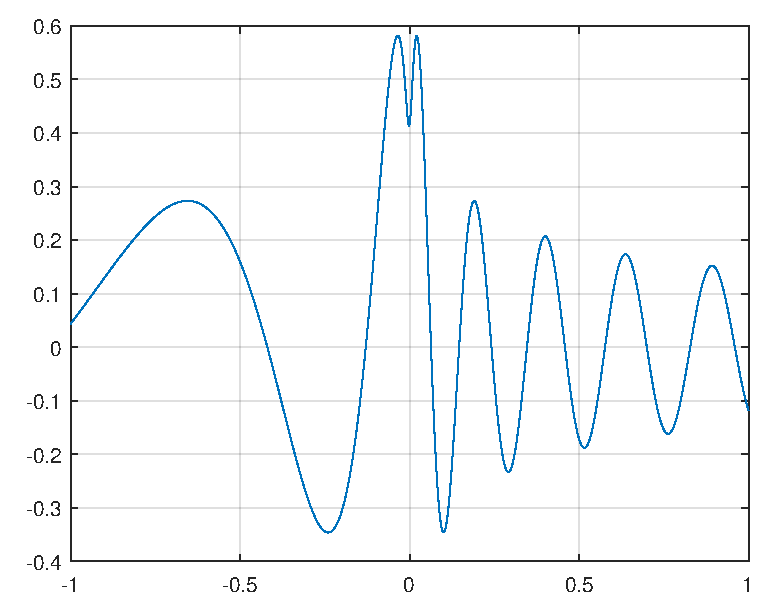
\includegraphics[width=0.495\textwidth]{gplot}
    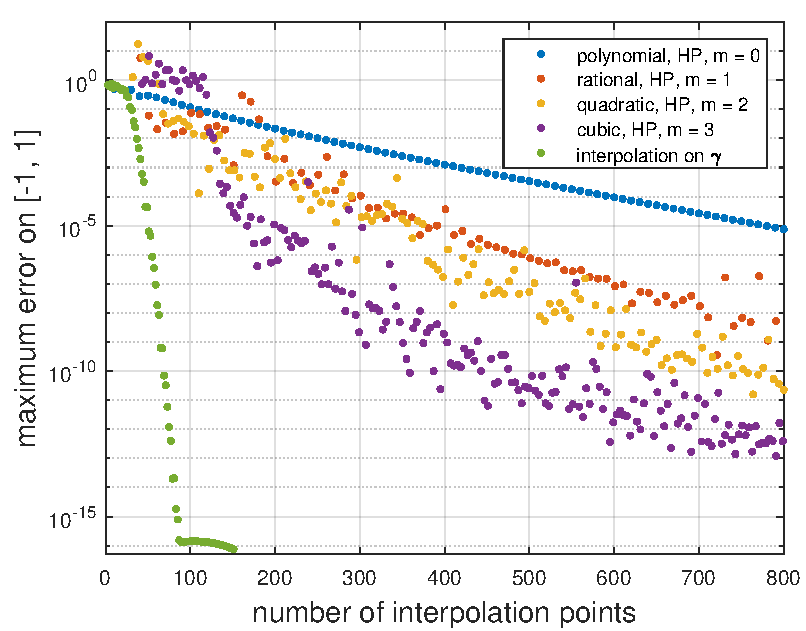
\includegraphics[width=0.495\textwidth]{fun_approx_bessel_example}
  \end{center} 
  \caption{Left: nearly singular function $g(t) = J_1(10t + 20\sqrt[3]{t^2 + \epsilon^2})$ with $\epsilon = 0.01$. Right:  rates of convergence of interpolants of $g$.  }\label{fig:funapproxex1}
\end{figure}

\subsection{Differential equations}

Functions of the form (\ref{eq:singforward}) and (\ref{eq:singinverse}) can also arise as solutions to differential equations. For example, 
\begin{align*}
f(t) = \sin(10t + 20\sqrt[3]{t^2 + \epsilon^2}), \qquad t \in [-1, 1],
\end{align*}
is the solution to the equation
\begin{align}
\frac{\mathrm{d}^2f}{\mathrm{d}t^2} + \left(10 + \frac{40t}{3\left(t^2 + \epsilon^2 \right)^{2/3}}  \right)^2 f = \cos(10t + 20\sqrt[3]{t^2 + \epsilon^2})\left( \frac{20(6\epsilon^2 - 2t^2)}{9\left(t^2 + \epsilon^2 \right)^{5/3}} \right),  \label{eq:DEex}
\end{align}
subject to, for example, $f(-1) = \sin(-10+ 20\sqrt[3]{1 +\epsilon^2})$ and $f(1) = \sin(10+ 20\sqrt[3]{1 +\epsilon^2})$.  If we set $y = y(t) = t$ and $x = x(t) = \sqrt[3]{t^2 + \epsilon^2}$, which defines the cubic curve (\ref{eq:cubiccurveex1}), then (\ref{eq:DEex}) becomes
\begin{align*}
x^5\frac{\mathrm{d}^2f}{\mathrm{d}t^2} + \frac{x}{9}\left(10x^2 + 40y  \right)^2 f = \frac{20}{9}\cos(10y + 20x)\left(6\epsilon^2 - 2y^2\right). 
\end{align*}
More generally, we consider equations of the form
\begin{align}
a_2(x,y) \frac{\mathrm{d}^2f}{\mathrm{d}t^2} + a_1(x,y) \frac{\mathrm{d}f}{\mathrm{d}t} + a_0(x,y)f = g(x,y),  \label{eq:2ndlin}
\end{align}
defined on a cubic curve and subject to initial or boundary conditions. 

Recall that $\mathbb{Y}_n$, $n \geq 0$ denotes the vector of orthonormalized basis functions of $\mathcal{V}_n$. Let
\begin{align*}
\mathbb{Y} = \left(
\begin{array}{c}
\mathbb{Y}_0\\
\mathbb{Y}_1 \\
\vdots
\end{array}
\right),
\end{align*}
then it follows from recurrence relations (\ref{eq:xrec}) and (\ref{eq:yrec}) that
\begin{align}
x\mathbb{Y} = \mathcal{J}_1 \mathbb{Y}, \qquad 
y\mathbb{Y} = \mathcal{J}_2 \mathbb{Y},\label{eq:jacops}
\end{align}
where $\mathcal{J}_1$ and $\mathcal{J}_2$ are the symmetric block-tridiagonal Jacobi operators
\begin{align*}
\mathcal{J}_{i} = \left( 
\begin{array}{c c c c c} 
 B_{0,i}                          & A_{0,i}   &         &     &         \\
A_{0,i}^{t}  & B_{1,i}   & A_{1,i} &     &         \\
&A_{1,i}^{t} & B_{2,i}   & A_{2,i} &       \\
 & & \ddots &\ddots & \ddots
\end{array}
\right), \qquad
i = 1, 2,
\end{align*}
and $A_{n,i}$, $B_{n,i}$ are defined below (\ref{eq:yrec}). We denote an expansion of the solution in the orthonormal basis on the cubic curve as
\begin{align*}
f = \wh f_0 \wh Y_0 + \wh f_{1,1} \wh Y_{1,1} + \wh f_{1,2} \wh Y_{1,2} + \sum_{k = 2}^{\infty}\left[ \wh f_{k,1} \wh Y_{k,1} + \wh f_{k,2} \wh Y_{k,2} +  \wh f_{k,3} \wh Y_{k,3}  \right] = \mathbb{Y}^{t}\,\widehat{\mathbf{f}}.
\end{align*} 
where $\widehat{\mathbf{f}}$ is the infinite vector of coefficients $\wh f_{k,i}$. From (\ref{eq:jacops}) it follows that
\begin{align*}
\left( \mathcal{J}_1 - x\mathcal{I}  \right)\partial_x \mathbb{Y} = \mathbb{Y}, \qquad  \left( \mathcal{J}_2 - y\mathcal{I}  \right)\partial_y \mathbb{Y} = \mathbb{Y},
\end{align*}
hence
\begin{align*}
\frac{\mathrm{d}}{\mathrm{d}t}\mathbb{Y} = \left[\frac{\mathrm{d}x}{\mathrm{d}t} \partial_x  + \frac{\mathrm{d}y}{\mathrm{d}t} \partial_y\right] \mathbb{Y} = \left[\frac{\mathrm{d}x}{\mathrm{d}t} \left( \mathcal{J}_1 - x\mathcal{I}  \right)^{-1}  + \frac{\mathrm{d}y}{\mathrm{d}t}\left( \mathcal{J}_2 - y\mathcal{I}  \right)^{-1}\right] \mathbb{Y} := \mathcal{D}_1\mathbb{Y},
\end{align*}
and
\begin{align*}
&\frac{\mathrm{d}^2}{\mathrm{d}t^2}\mathbb{Y} = \left[\frac{\mathrm{d}^2x}{\mathrm{d}t^2} \partial_x  + \frac{\mathrm{d}^2y}{\mathrm{d}t^2} \partial_y\right] \mathbb{Y} + \left[\frac{\mathrm{d}x}{\mathrm{d}t} \partial_x  + \frac{\mathrm{d}y}{\mathrm{d}t} \partial_y\right]^2 \mathbb{Y} = \\
&\left\lbrace\left[\frac{\mathrm{d}^2x}{\mathrm{d}t^2} \left( \mathcal{J}_1 - x\mathcal{I}  \right)^{-1}  + \frac{\mathrm{d}^2y}{\mathrm{d}t^2}\left( \mathcal{J}_2 - y\mathcal{I}  \right)^{-1}\right] + \left[\frac{\mathrm{d}x}{\mathrm{d}t} \left( \mathcal{J}_1 - x\mathcal{I}  \right)^{-1}  + \frac{\mathrm{d}y}{\mathrm{d}t}\left( \mathcal{J}_2 - y\mathcal{I}  \right)^{-1}\right]^2\right \rbrace\mathbb{Y} \\
&:=\mathcal{D}_2\mathbb{Y}.
\end{align*}
It follows that in coefficient space, (\ref{eq:2ndlin}) can be represented as
\begin{align*}
\left[a_2(\mathcal{J}_1,\mathcal{J}_2)\mathcal{D}_2^{t} + a_1(\mathcal{J}_1,\mathcal{J}_2)\mathcal{D}_1^{t} + a_0(\mathcal{J}_1,\mathcal{J}_2)\right]\widehat{\mathbf{f}} = \widehat{\mathbf{g}}.
\end{align*}







\begin{thebibliography}{99}

\bibitem{DX} 
        C. F. Dunkl and Y. Xu,
        \textit{Orthogonal Polynomials of Several Variables}
        Encyclopedia of Mathematics and its Applications \textbf{81},
         Cambridge University Press, Cambridge, 2001.
         
\bibitem{gautschi}
        W. Gautschi,
  \textit{Orthogonal Polynomials: Computation and Approximation},
  Oxford University Press, 2004.
  
\bibitem{gonnet}
  P. Gonnet, R. Pach\'on, and L.N. Trefethen,
  Robust rational interpolation and least-squares,
  \textit{Elect. Trans. Numer. Anal.},
  38 (2011), 146--167.
   
 \bibitem{Ko}
          N. Koblitz, 
          Introduction to elliptic curves and modular forms, 
          Springer, 1993.         

\bibitem{OX1}
       S. Olver and Y. Xu,
       Orthogonal structure on a wedge and on the boundary of a square, 
       \textit{Found. Comp. Math.}, 19 (2019), 561--589.

\bibitem{OX2}
       S. Olver and Y. Xu,
       Orthogonal structure on a quadratic curve, 
       arXiv:1807.04195.
       
\bibitem{pachon}
R. Pach\'on, P. Gonnet, and J. Van Deun,
Fast and stable rational interpolation in roots of unity and Chebyshev points,
\textit{SIAM J. Numer. Anal.},
50 (2012), 1713--1734.
       
\end{thebibliography}
\end{document}
 